%!TEX root = ../Thesis.tex
%! Author = JB
%! Date = 22.05.2020


\section{Entity-Relationship Diagramm \textcolor{blue}{[Jonathan Brockhausen]}}

In \cref{fig:erd} ist das zugrundeliegende Entity-Relationship Diagramm dargestellt.

\begin{figure}[h!!]
    \centering
    \begin{minipage}[t]{1\textwidth}
        \caption{ERD des Projekts}
        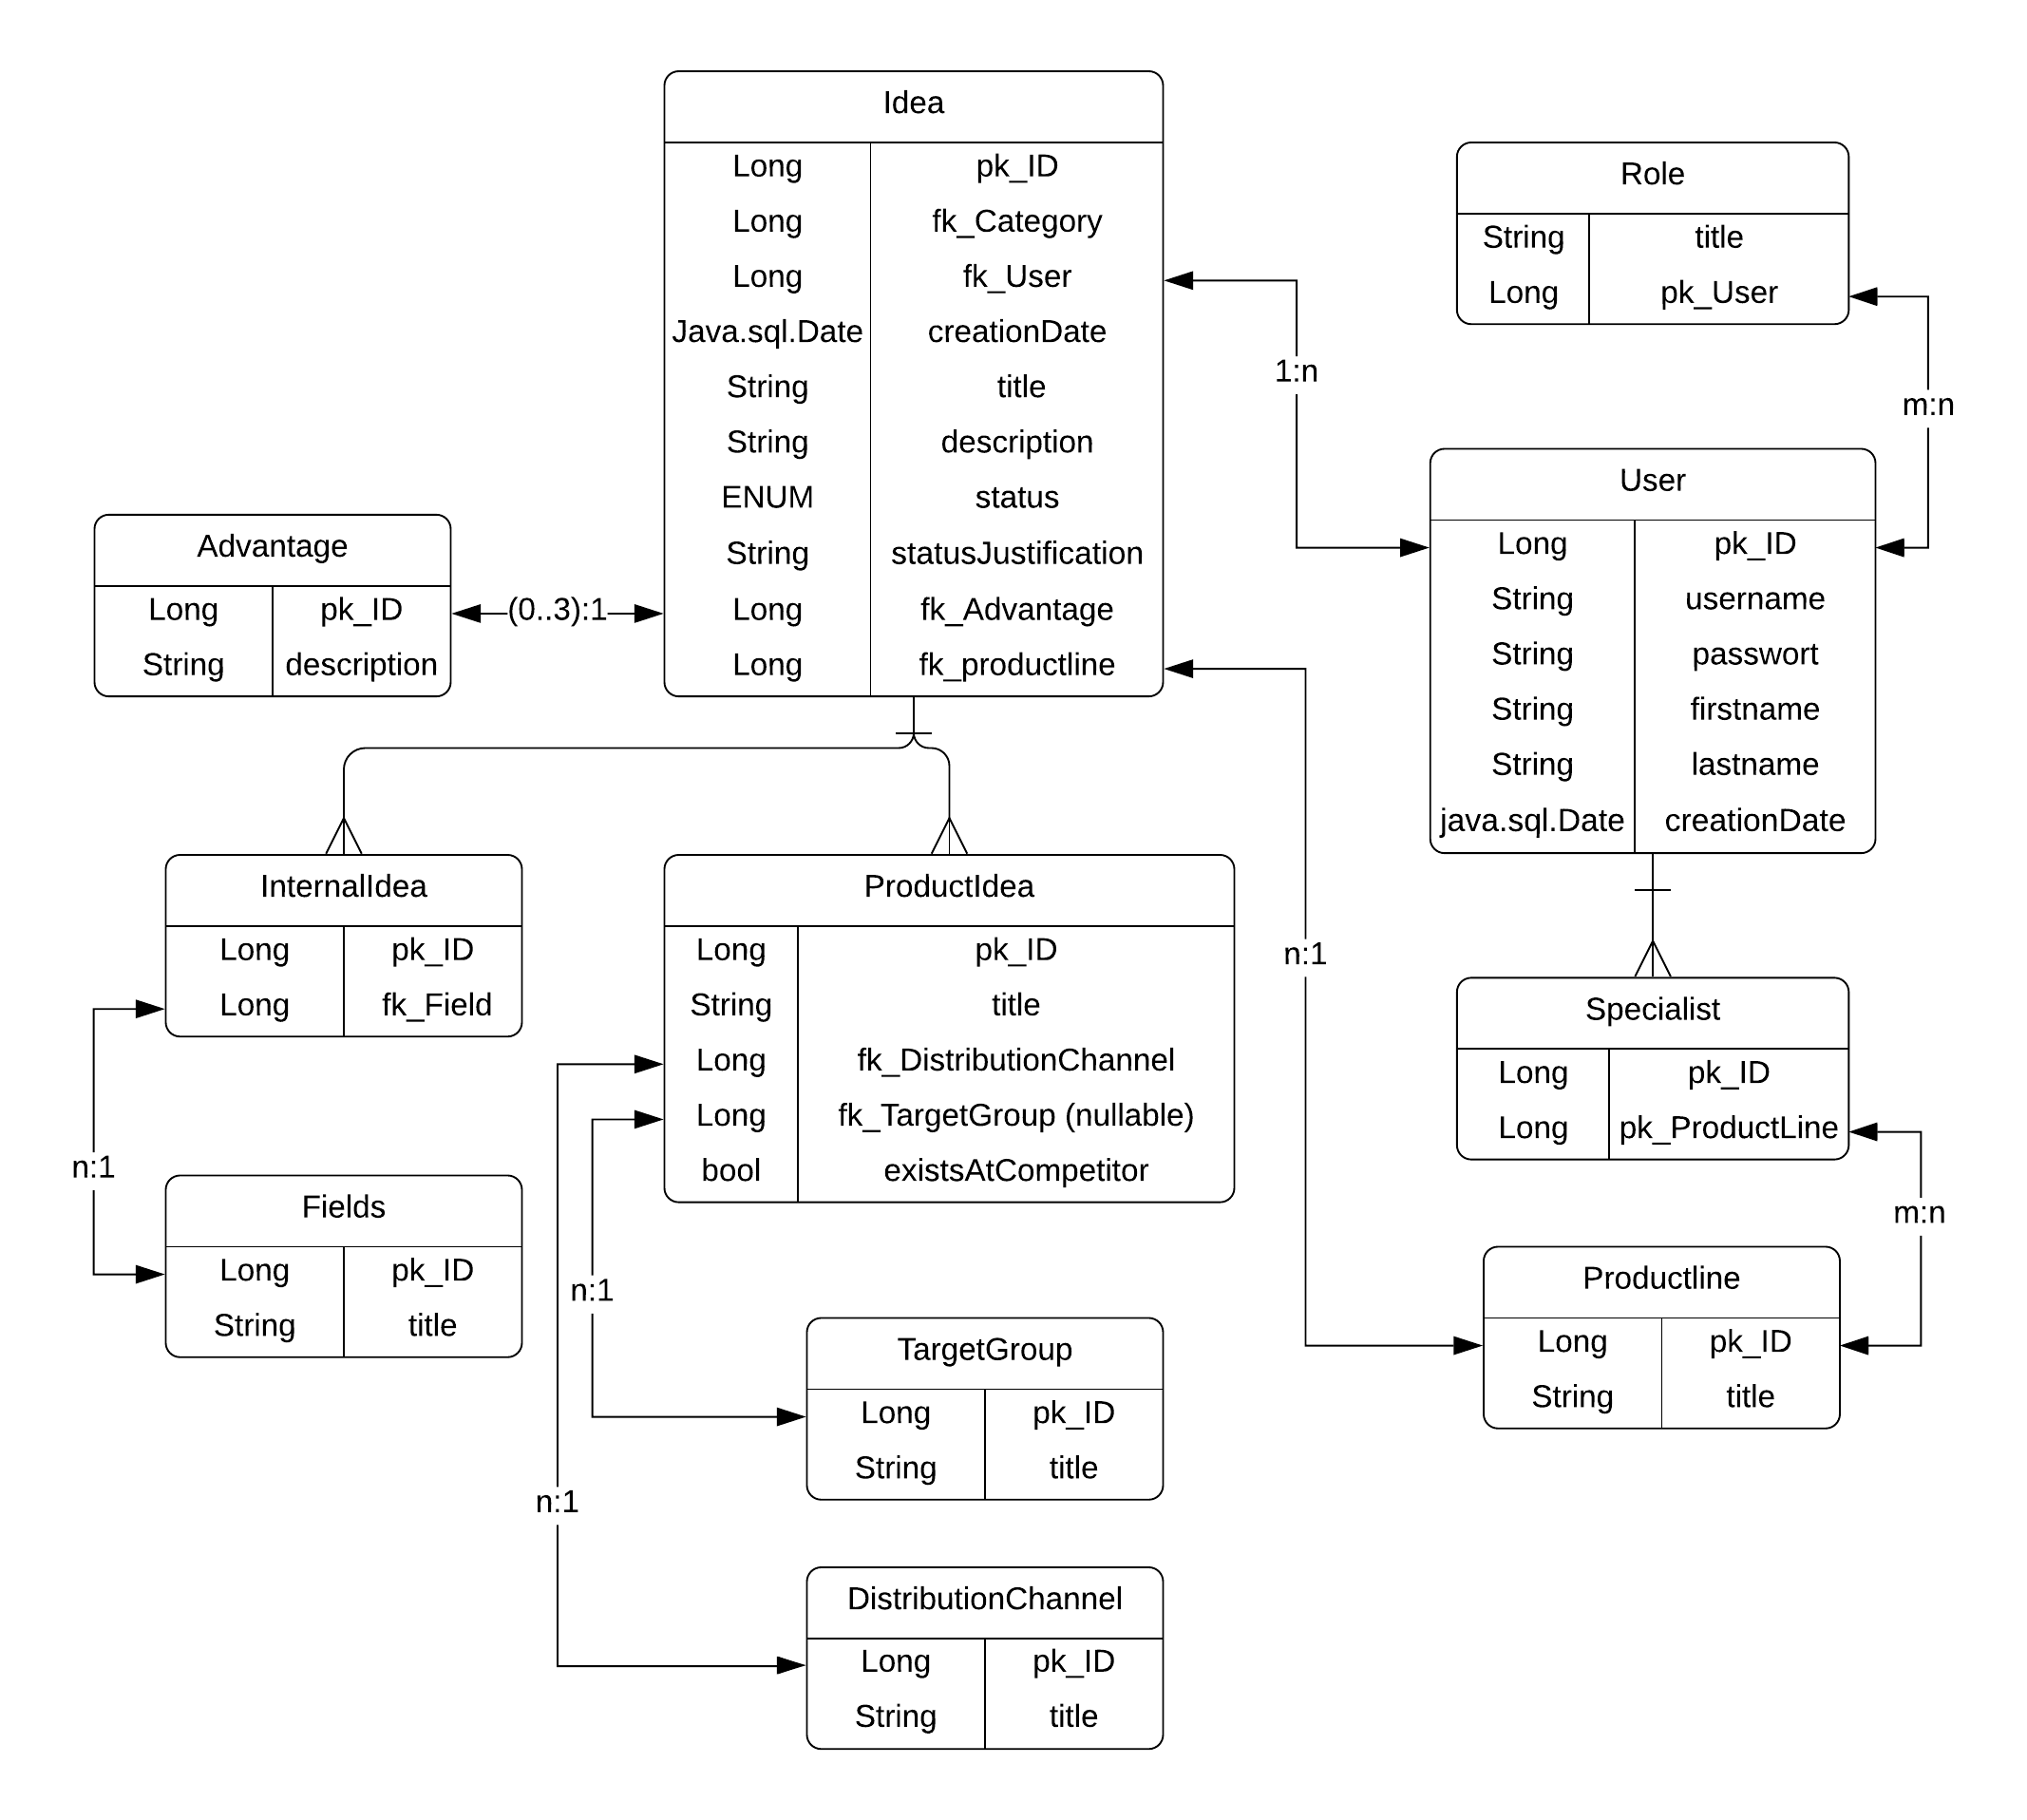
\includegraphics[width=1\textwidth]{img/erd.png}\\
        \source{Eigene Darstellung}
        \label{fig:erd}
    \end{minipage}
\end{figure}

Die Datenstruktur wurde auf Basis dieses Entity-Relationship Diagramms implementiert. Im Folgenden werden einige Design-Entscheidungen erläutert.\\
\textbf{Zuordnung von Fachspezialisten und Ideen}\\
Um die automatische Zuordnung von Fachspezialisten zu Ideen umzusetzen, haben wir die Produktsparte als Zuordnungskriterium gewählt.
Die Klasse des Fachspezialisten erbt von der Klasse des Benutzers mit der zusätzlichen Eigenschaft, dass ihm eine oder mehrere Produktsparten zugewiesen sind.
Einer Produktsparte können mehrere Fachspezialisten zugeordnet sein. Mit dieser m:n-Beziehung erreicht das Programm die größtmögliche Flexibilität.
Jeder Idee (Intern und Produkt) ist eine Produktsparte zugeordnet. Aus den Projektanforderungen ergeben sich mehrere Produktsparten, die bei der Auslieferung bereits vorhanden sind.
Da interne Ideen gemäß der Anforderungen keine Produktsparte besitzen, bekommen Sie die dem Benutzer verborgene Produktsparte \glqq{}INTERNAL\grqq{} zugewiesen. Diese ermöglicht für interne Ideen dieselbe Logik zu verwenden.
Durch diese Umsetzung ist auch eine Erweiterung um weitere Ideenkategorien ohne Änderungen am übrigen Programm möglich.\\
\textbf{Umsetzung von Status}\\
Wir haben uns dagegen entschieden, den Status in eine eigene Entität im Sinne des ERD auszulagern.
Erweiterungen und Änderungen der Status im Echtbetrieb erfordern ohnehin an einigen Stellen Änderungen in der Programmlogik, weshalb es keinen Sinn macht, Status als Datenbank-Entitäten umzusetzen.\\
\textbf{Vererbung von Ideen zu interne und Produktidee}\\
Die Struktur der Vererbung von Ideen ermöglicht es, weitere Kategorien von Ideen anzulegen ohne die bestehenden zu verändern. Hierbei können bereits angelegte Eigenschaften genutzt und neue hinzugefügt werden. 